\documentclass[10pt]{beamer}

% Beamer style
%\usetheme[secheader]{Madrid}
% \usetheme{CambridgeUS}
\useoutertheme{infolines}
\usecolortheme[rgb={0.65,0.15,0.25}]{structure}
% \usefonttheme[onlymath]{serif}
\beamertemplatenavigationsymbolsempty
%\AtBeginSubsection

% Packages
%\usepackage[french]{babel}
\usepackage[latin1]{inputenc}
\usepackage{color}
\usepackage{xspace}
%\usepackage{dsfont, stmaryrd}
\usepackage{amsmath, amsfonts, amssymb}
\usepackage{epsfig}
\usepackage{url}
\usepackage{/home/robin/LATEX/Biblio/astats}
%\usepackage[all]{xy}
\usepackage{graphicx}

% Commands
\definecolor{darkred}{rgb}{0.65,0.15,0.25}
\newcommand{\emphase}[1]{\textcolor{darkred}{#1}}
% \newcommand{\emphase}[1]{{#1}}
\newcommand{\paragraph}[1]{\textcolor{darkred}{#1}}
\newcommand{\refer}[1]{{\footnotesize{\textcolor{gray}{[{\cite{#1}}]}}}}
\newcommand{\Refer}[1]{{\footnotesize{\textcolor{gray}{[{#1}]}}}}
\renewcommand{\newblock}{}

% Symbols
\newcommand{\dd}{\xspace\text{d}}
\newcommand{\Esp}{\mathbb{E}}
\newcommand{\Ibb}{\mathbb{I}}
\newcommand{\Cov}{\mathbb{C}\text{ov}}
\newcommand{\Var}{\mathbb{V}}
\newcommand{\Hcal}{\mathcal{H}}
\newcommand{\Mcal}{\mathcal{M}}
\newcommand{\Ncal}{\mathcal{N}}
\newcommand{\pa}{\text{pa}}
\newcommand{\ra}{\emphase{\mathversion{bold}{$\rightarrow$}~}}
\newcommand{\Scal}{\mathcal{S}}

% Directory
\newcommand{\figmixt}{/home/robin/ENSEIGN/COURS/MELANGE}
\newcommand{\figbma}{/home/robin/RECHERCHE/RUPTURES/MELANGE/Exemples/Grippe}
\newcommand{\fignet}{../FIGURES}
\newcommand{\figeco}{/home/robin/RECHERCHE/ECOLOGIE/EXPOSES/FIGURES}
%\newcommand{\figmotif}{/home/robin/RECHERCHE/RESEAUX/Motifs/FIGURES}


%====================================================================
%====================================================================

%====================================================================
%====================================================================
\begin{document}
%====================================================================
%====================================================================

%====================================================================
\frame{\frametitle{Diversity of a trait}

  $$
  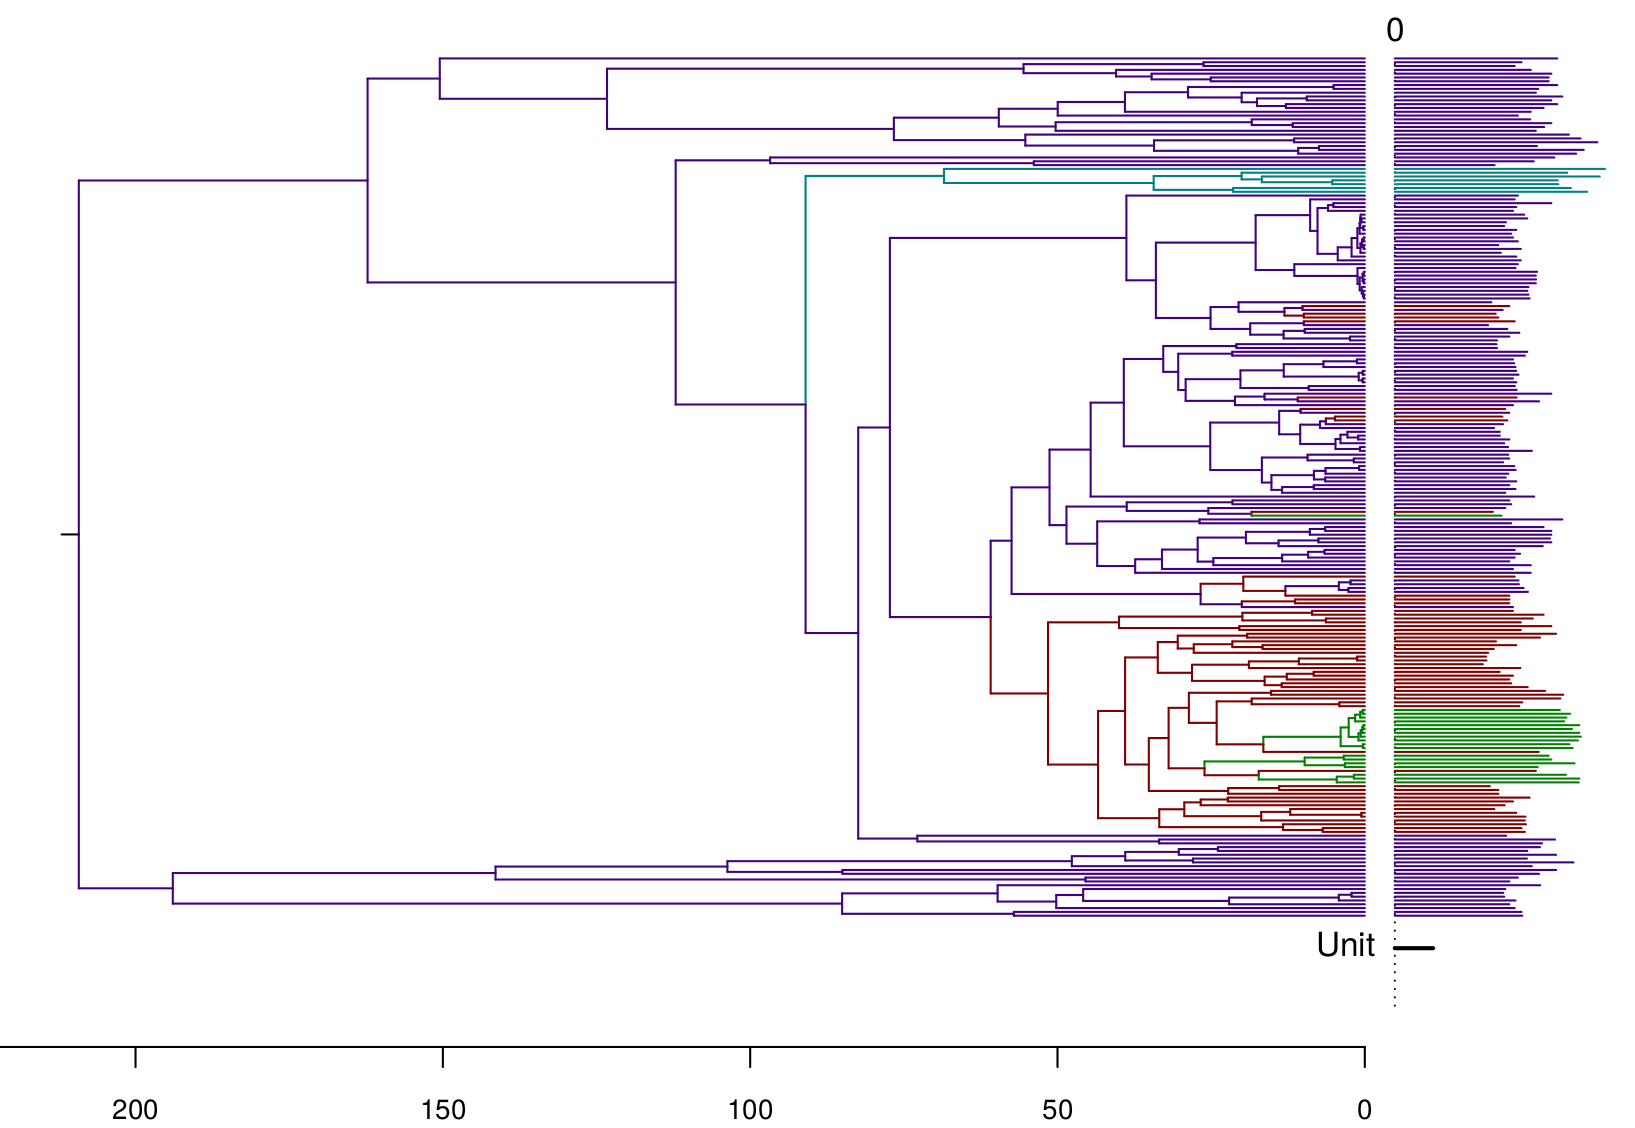
\includegraphics[width=.8\textwidth, clip=]{../FIGURES/plot_data_chel-intro-SR}
  $$
  \refer{JSA11}
  }

%====================================================================
\frame{\frametitle{Evolution of a trait}

  \begin{tabular}{cc}	
    \hspace{-0.1\textwidth}
    \begin{tabular}{c}
    Phylogenetic tree \\ ~\\
    \includegraphics[width=.5\textwidth, clip=]{../FIGURES/plot_tree_tims_2-1}
    \end{tabular}
    &
    \hspace{-0.05\textwidth}
    \begin{tabular}{c}
    Process on the tree  \\ ~\\
    \includegraphics[width=.5\textwidth, clip=]{../FIGURES/plot_BM_sim_2-1}
    \end{tabular}
  \end{tabular}
  }

%====================================================================
\frame{\frametitle{Introducing shifts}

  \begin{tabular}{cc}	
    \hspace{-0.1\textwidth}
    \begin{tabular}{c}
    Phylogenetic tree \\ ~\\
    \includegraphics[width=.5\textwidth, clip=]{../FIGURES/plot_tree_tims_shift-1}
    \end{tabular}
    &
    \hspace{-0.05\textwidth}
    \begin{tabular}{c}
    Process on the tree  \\ ~\\
    \includegraphics[width=.5\textwidth, clip=]{../FIGURES/plot_BM_sim_shit-1} \\	
    clusters: $(A, B, D)$ / $(C, E)$
    \end{tabular}
  \end{tabular}
}

%====================================================================
\frame{\frametitle{Identifiability: Parsimony}

  \begin{tabular}{p{.25\textwidth}p{.05\textwidth}p{.25\textwidth}p{.05\textwidth}p{.25\textwidth}}
    \begin{tabular}{c}
    \includegraphics[width=0.15\textwidth]{../FIGURES/colours_1_nodes_gray} \\
    2 colors \\ ~
    \end{tabular}
    & 
    \begin{tabular}{c}
    $:$
    \end{tabular}
    & 
    \begin{tabular}{c}
    \includegraphics[width=0.15\textwidth]{../FIGURES/colours_2_nodes_gray} \\
    non \\
    parsimonious
    \end{tabular}
    & 
    \begin{tabular}{c}
    $<$
    \end{tabular}
    & 
    \begin{tabular}{c}
    \includegraphics[width=0.15\textwidth]{../FIGURES/colours_3_nodes_gray} \\
    parsimonious: \\ 
    no homoplasy 
    \end{tabular}
  \end{tabular}
}

%====================================================================
\frame{\frametitle{Identifiability: Equivalence}

  \begin{tabular}{p{.25\textwidth}p{.05\textwidth}p{.25\textwidth}p{.05\textwidth}p{.25\textwidth}}
    \begin{tabular}{c}
    \includegraphics[width=0.15\textwidth]{../FIGURES/colours_bis_1_nodes_gray} \\
    3 colors
    \end{tabular}
    & 
    \begin{tabular}{c}
    $:$
    \end{tabular}
    & 
    \begin{tabular}{c}
    \includegraphics[width=0.15\textwidth]{../FIGURES/colours_bis_2_nodes_gray} \\
    parsimonious
    \end{tabular}
    & 
    \begin{tabular}{c}
    $\sim$
    \end{tabular}
    & 
    \begin{tabular}{c}
    \includegraphics[width=0.15\textwidth]{../FIGURES/colours_bis_3_nodes_gray} \\
    parsimonious
    \end{tabular}
  \end{tabular}

}

%====================================================================
\frame{ \frametitle{Example of equivalent scenarios}

  OU model: this 5 configurations only count for 1.
  $$
  \includegraphics[width=.8\textwidth]{../FIGURES/plot_parsimony-1}
  $$
}

%====================================================================
\frame{ \frametitle{Chelonia turtles}

  \only<1>{
\begin{columns}
\begin{column}{0.55\textwidth}
\begin{minipage}[c][\textheight][c]{\linewidth}
\vskip -1 cm
    \includegraphics[width=\linewidth]{../FIGURES/plot_chel_data1-1} \\
    {\footnotesize Colors: habitats.\\ Boxes: selected EM regimes.}
\end{minipage}
\end{column}
\begin{column}{0.45\textwidth}
\begin{minipage}[t][.6\textheight][c]{\linewidth}
\end{minipage}
\end{column}
\end{columns}
}
\only<2>{
\begin{columns}
\begin{column}{0.55\textwidth}
\begin{minipage}[c][\textheight][c]{\linewidth}
\vskip -1 cm
    \includegraphics[width=\linewidth]{../FIGURES/plot_chel_data-1} \\
    {\footnotesize Colors: habitats.\\ Boxes: selected EM regimes.}
\end{minipage}
\end{column}
\begin{column}{0.45\textwidth}
\begin{minipage}[t][.6\textheight][c]{\linewidth}
\vskip - 4 cm
\includegraphics[width=0.5\textwidth]{../FIGURES/Chelonia_mydas.jpg} \\
{\footnotesize Chelonia mydas}
\end{minipage}
\end{column}
\end{columns}
}
\only<3>{
\begin{columns}
\begin{column}{0.55\textwidth}
\begin{minipage}[c][\textheight][c]{\linewidth}
\vskip -1 cm
\includegraphics[width=\linewidth]{../FIGURES/plot_chel_data3-1}  \\
{\footnotesize Colors: habitats.\\ Boxes: selected EM regimes.}
\end{minipage}
\end{column}
\begin{column}{0.45\textwidth}
\begin{minipage}[t][.6\textheight][c]{\linewidth}
\includegraphics[width=0.5\textwidth]{../FIGURES/Geochelone_nigra_abingdoni.jpg} \\
{\footnotesize Geochelone nigra abingdoni}
\end{minipage}
\end{column}
\end{columns}
}
\only<4>{
\begin{columns}
\begin{column}{0.55\textwidth}
\begin{minipage}[c][\textheight][c]{\linewidth}
\vskip -1 cm
\includegraphics[width=\linewidth]{../FIGURES/plot_chel_data5-1} \\
{\footnotesize Colors: habitats.\\ Boxes: selected EM regimes.}
\end{minipage}
\end{column}
\begin{column}{0.45\textwidth}
\begin{minipage}[t][.6\textheight][c]{\linewidth}
\vskip - 4 cm
\includegraphics[width=0.5\textwidth]{../FIGURES/Dudhwalive_chitra.jpg} \\
{\footnotesize Chitra indica}
\end{minipage}
\end{column}
\end{columns}
}
\only<5>{
\begin{columns}
\begin{column}{0.55\textwidth}
\begin{minipage}[c][\textheight][c]{\linewidth}
\vskip -1 cm
\hspace{.025\textwidth}
\includegraphics[width=\linewidth]{../FIGURES/plot_chel_data4-1} \\
{\footnotesize Colors: habitats.\\ Boxes: selected EM regimes.}
\end{minipage}
\end{column}
\begin{column}{0.5\textwidth}
\begin{minipage}[t][.6\textheight][c]{\linewidth}
\vskip - 3 cm
{\footnotesize
\begin{table}[!ht]
\begin{center}
\begin{tabular}{l|c|c}
\hline
  & Habitat & EM\\ \hline
Nb shifts & 16 & 5\\ \hline
Nb regimes & 4 & 6\\ \hline
$\log P$ & -135.56 & -97.59\\ \hline
$\ln 2 / \alpha$ (\%) & 7.83 & 5.43\\ \hline
$\gamma^2$ & 0.35 & 0.22\\ \hline
CPU (mn) & 1.25 & 134.49\\ \hline
\end{tabular}
\end{center}
\end{table}
}
\end{minipage}
\end{column}
\end{columns}
}
}

%====================================================================
\frame[allowframebreaks]{ \frametitle{References}

\nocite{BMR16} 

{\tiny
  \bibliography{/home/robin/Biblio/BibGene}
  \bibliographystyle{/home/robin/LATEX/Biblio/astats}
  %\bibliographystyle{plain}
  }
}

 
%====================================================================
%====================================================================
\end{document}
%====================================================================
%====================================================================

  \begin{tabular}{cc}
    \begin{tabular}{p{.5\textwidth}}
    \end{tabular}
    & 
    \hspace{-.02\textwidth}
    \begin{tabular}{p{.5\textwidth}}
    \end{tabular}
  \end{tabular}

